\section{Model/Implementation Details}\label{sec:Model-Implem-Details}



\subsection{Programming Language}
I plan to program this in C++, as that is one of the languages that I am more familiar with (along with C), and it is also one of the main languages that is used in physics nowadays. Further, interpreted languages like Python usually end up being too slow for intense simulations like this. For this project it likely would have been fine, especially if I was able to implement anything on the GPU, but C++ has GPU programming toolets anyway (like CUDA), though a bit more cumbersome to use. Further, the existing tools I plan to use for my project have their main API in C++ with the Python version usually being more of a side-thought, so it is more favorable in that regard as well.



\subsection{Other Tools and Frameworks}

There are two external tools that I know I will be using, and those are the Gnuplot and LHAPDF. Gnuplot is a simple command-line tool used for plotting data, and it will allow me to visualize results very easily and nicely, and have them be comparable to results from other frameworks.

\textsc{LHAPDF} is a package used to interface with \textit{parton distribution functions} (PDFs). These are used to describe the structure of the proton, specifically the probability of finding different quarks within the proton given some momentum fraction $x$. This has to be done this way, by which I mean interfacing with some external package, because the PDFs are not able to be calculated on their own; they have to be determined from experiment and encoded in data file. This is required in the calculational side of things. There is one caveat with this library, and it seems that it can only be built on Unix-like distributions.

\subsubsection{The GNU Scientific Library (GSL)}

There are a number of mathematical routines that are required to implement this simulation. There are few enough that I would likely be able to program them on my own, but I would like to avoid spending too much time on such subroutines since they are not the main focus of the project. Additionally, I'd like any of my naive implementations of the algorithms to not interfere with the main simulation process. Therefore, at least at first, I may rely on the GNU Scientific Library (GSL). This is C library providing a large number of subroutines, most importantly numerical integration, root-finding, and others. It's a moderately large library, and as I'd only be using a few of the subroutines, I'd like to eventually phase it out with some of my own implementations of the algorithms. Monte Carlo integration, for instance, is something I've already implemented. However, like I just mentioned, at least for now it will be a dependency so I can focus on the core functionality.


\subsection{Model Structure/Diagrams}

UML diagrams will be shown shortly, but I first give a prose version of how the model will be laid out and how the code is structured. Inspiration is taken from the \textsc{Pythia8} library. The name of my own library will be called \textsc{ColSim}, short for Collision-Simulation.

The basic directory structure for the project is organized like so:

\dirtree{%
  .1 CMakeLists.txt.
  .1 Source.
  .2 CMakeLists.txt.
  .2 Core.
  .3 CMakeLists.txt.
  .3 inc.
  .4 ColSim.
  .5 Core.
  .6 \ldots.
  .3 src.
  .4 \ldots.
  .2 Math.
  .2 Physics.
  .2 Plotting.
  .2 \ldots.
  .1 res.
  .2 config.in.
  .2 manual.
  .3 \ldots.
  .1 share.
  .2 cmake.
  .3 FindLHAPDF.cmake.
  .3 FindGSL.cmake.
  .1 Tests.
  .2 CMakeLists.txt.
  .2 Test1.
  .3 CMakeLists.txt.
  .3 main.cpp.
}

From the root directory, there is a global CMake file to which the other folders are added as subdirectories. The \mintinline{cfg}{share} folder contains other CMake files used to aid in finding the host system's versions of LHAPDF and GSL. The \mintinline{cfg}{Tests} contain at the moment only one test equipped with a main function with which to test the functionality of the main program. The \mintinline{cfg}{Source} contains all of the subdirectories of the project, where different functionality can be contained. For instance, all functionality related to the interface with Gnuplot is contained within the \mintinline{cfg}{Plotting} directory. Each of these directories are equipped with a CMake file, and include, and source directory in which headers and C++ source files are located. Lastly, back in the root directory of the project is the \mintinline{cfg}{res} folder containing the config file and some other files related to the project documentation contained in the \mintinline{cfg}{manual} subdirectory.

In terms of the actual model implementation, the basics start in the \mintinline{cfg}{Core} subproject, in which all of the core functionality that is not dependent on anything else but the standard library or other Core elements is implemented. For instance, the logger that logs to standard out/err and/or a dedicated log file is stored here, as well as some utility functions for strings and vectors which, for some reason, aren't present in the STL. Most importantly is the class \mintinline{cpp}{ColSimBase}, which contains a static pointer to the logger and other things like settings/options specified within the configuration file. Every other class that I make in the rest of the project will inheret from this class so that they have access to these things.

The one exception is the \mintinline{cfg}{Math} subproject, which contains all of the mathematical subroutines used in the simulation. These function signatures take inspiration from GSL. Since they are purely mathematical and have no relation to any specific physical process, they don't need to inherent from anything.

The \mintinline{cfg}{Physics} subproject is the most important, and contains all of the physics-related code relevent for the simulation. For instance, all physical constants are defined in a header file in this subproject, as well as classes for all of the different types of processes, along with the master \mintinline{cpp}{ColSim} class used to actually create the process, read in the configuration file, and execute the relevant subroutines.

As just mentioned, each process has its own class, inhereted from the main \mintinline{cpp}{ProcessBase} class, which provides members and functions that every class should use such as methods to determine phase space points and methods to simply return the evaluation of the partonic cross section at a specified phase space point. The full parton-shower core functionality has yet to be implemented, but it will follow a similar style, where each type of process will be sectioned off into its own class that inherents from some overall \mintinline{cpp}{PartonShowerBase} class.

Also contained in the \mintinline{cpp}{Physics} library are classes for kinematics such as the \mintinline{cpp}{FourVector} class, from which specific four vectors like the four-momentum and four-position are implemented. These contain some of the kinematic information of each particle.

Once the event generation starts and the cross section is computed, events will be created and stored in the \mintinline{cpp}{Event} class, which will contain a record of all the particles, represented by the \mintinline{cpp}{Particle} class. Each particle will contain its own momentum, any other necessary kinematical variables, as well as identifying information that ties it to its event. For emitted particles during the parton showering step, additional information will need to be contained tying the emitted particle to its ``parent'' particle.


\subsection{Graphical Diagrams}

\begin{figure}[ht]
  \centering
  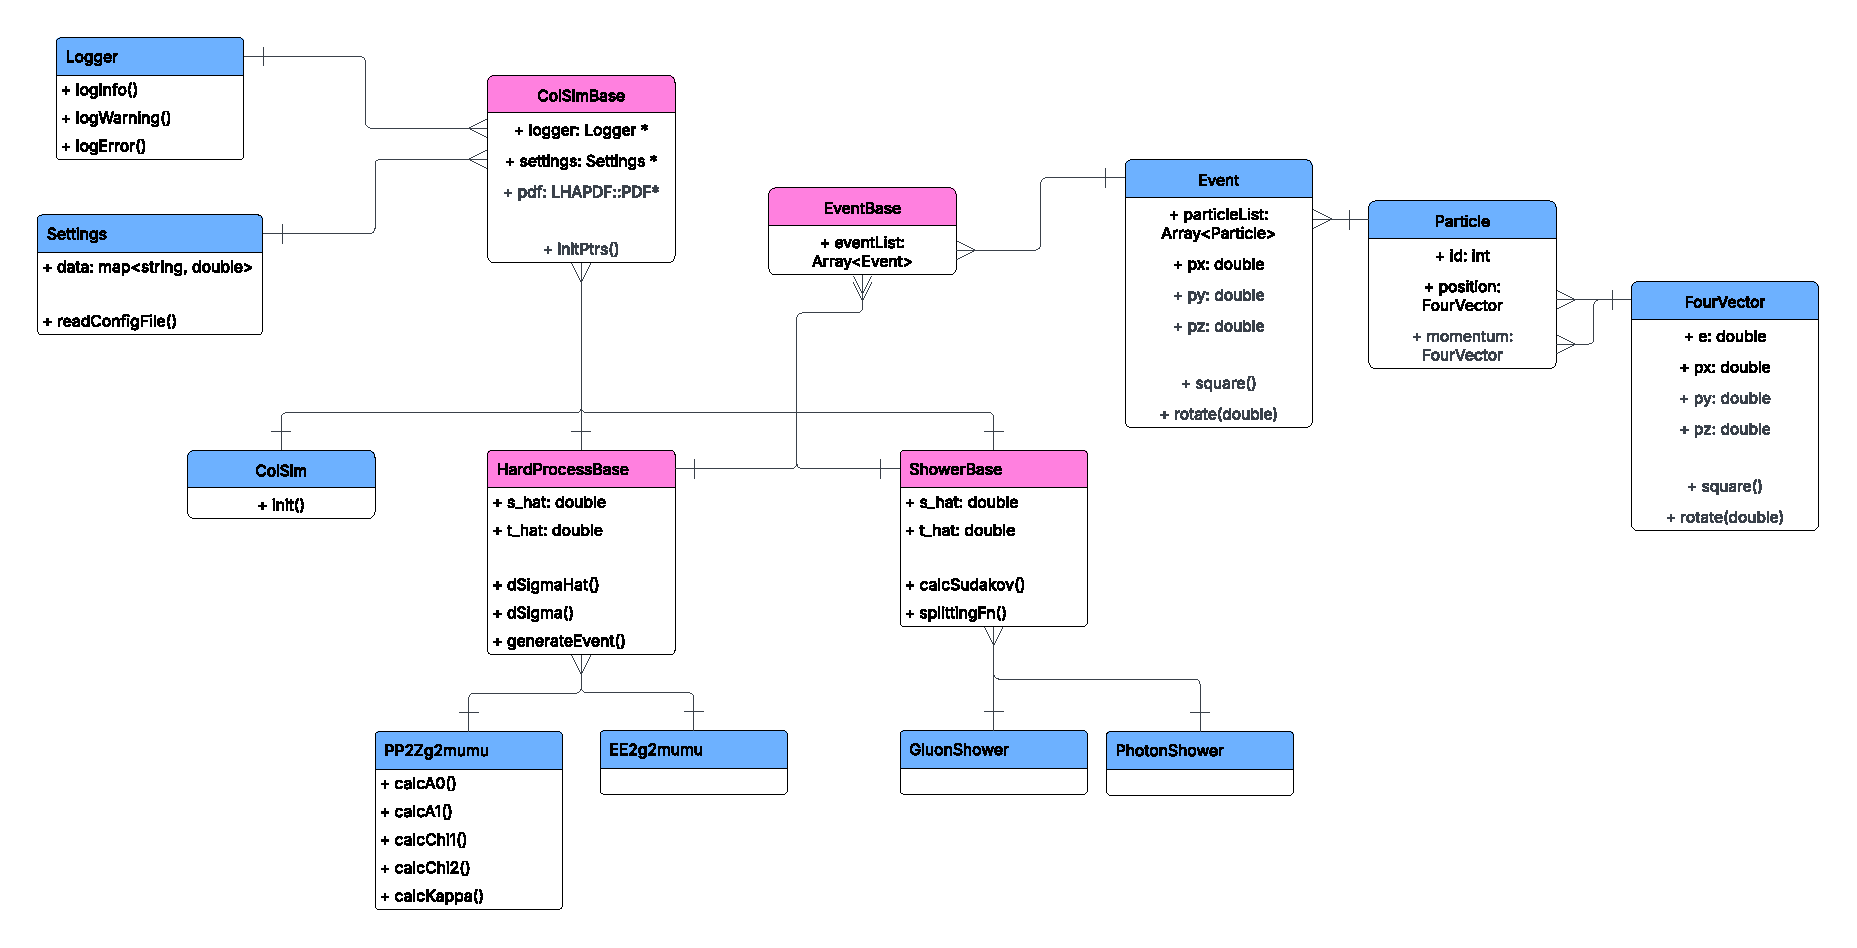
\includegraphics[width=0.9\linewidth]{./res/Images/ColSim.pdf}
  \caption{Basic UML diagram describing the interaction/relationships between the different classes.}
  \label{fig:uml}
\end{figure}


Given in Fig.~\ref{fig:uml} is the current status of the program in terms of the interactions/relationships between the different classes expressed as a UML diagram, with the exception of the \mintinline{cfg}{Math} subproject, since, as mentioned earlier, it is separate from the physics processes. This is simply a graphical representation of what has already been described, so I won't discuss much about it, apart from the fact that some classes don't have fully fleshed out members/methods. The current results of the progam, for instance, were retrieved via directly using the methods in the \mintinline{cpp}{PP2Zg2mumu} class without first going through the main \mintinline{cpp}{ColSim} class. One more processes start being fully implemented, this more object-oriented structure will start to take hold.



\subsection{Current Challenges}

At the moment, one of the largest challenges is that all of the documentation on the internet for event generators like these is either extremely low-level, spanning hundred of pages and often jumping right to NLO or NNLO implementations of things, or it is extremely high-level, where it is formed almost like a tutorial of sorts, and the end product is the implementation of one single process at one order with a very small subset of observable results. These tutorials have provided a fantastic source of some basic implementation for some specific processes, but any sort of generality is left to me.

Fortunately, there is a professor here at KSU who is quite familiar with these tools, and has actually worked quite a lot on \textsc{Herwig7}. He works in an adjacent department to the one I do research in, and I have had two classes with him and had many discussions on things after/before class, so he will be a very approachable resource for information on this topic.



%%% Local Variables:
%%% mode: LaTeX
%%% TeX-master: "../../Report"
%%% End:
